%\documentclass[notes,xcolor={x11names,dvipsnames,svgnames},compress]{beamer}
\documentclass[notes,xcolor={x11names,dvipsnames,svgnames},compress]{beamer}

\usepackage{lmodern}
\usepackage[utf8]{inputenc}
\usepackage[T1]{fontenc}
\usepackage{graphicx}
\usepackage{animate}
\usepackage{booktabs}
\usepackage{tikz}
\usepackage{amsmath}
\usepackage{empheq}
\usepackage{pgf}
\usepackage{import}
%\usepackage{media9}
%\usepackage{movie15}
\usepackage{multimedia}
\usepackage{hyperref}
\usepackage{tabularx}
\usepackage{verbatim}
\usepackage{listings}
\usepackage{tikz}

\newsavebox{\picbox}

\newcommand{\cutpic}[3]{
  \savebox{\picbox}{\includegraphics[width=#2]{#3}}
  \tikz\node [draw, rounded corners=#1, line width=4pt,
    color=white, minimum width=\wd\picbox,
    minimum height=\ht\picbox, path picture={
      \node at (path picture bounding box.center) {
        \usebox{\picbox}};
    }] {};}
%\usepackage{xmpmulti}

%\usepackage{natbib}
%\usepackage{pgfpages}
%\setbeameroption{notes on second screen=left}

\usetikzlibrary{arrows}
\usetikzlibrary{decorations.pathmorphing}

\useoutertheme[subsection=false,shadow]{miniframes}
\useinnertheme{default}

\AtBeginSection[]{
  \begin{frame}
  \vfill
  \centering
  \begin{beamercolorbox}[sep=8pt,center,shadow=true,rounded=true]{title}
    \usebeamerfont{title}\insertsectionhead\par%
  \end{beamercolorbox}
  \vfill
  \end{frame}
}

%\usefonttheme{serif}
%\usepackage{palatino}
%\usepackage{pifont}

%\usefonttheme{professionalfonts}
%\usefonttheme{serif}
%\usepackage{uarial}
\renewcommand{\familydefault}{\sfdefault}

%\usepackage{fontspec}
%\setmainfont{Helvetica Neue}
%\setmainfont{Arial}

\definecolor{sand}{RGB}{242,240,218}
\definecolor{romi}{RGB}{53,168,100}
\setbeamerfont{title like}{shape=\scshape}
\setbeamerfont{frametitle}{shape=\scshape}

\setbeamercolor*{lower separation line head}{bg=sand}
\setbeamercolor*{palette tertiary}{fg=black,bg=black!10}
\setbeamercolor*{palette quaternary}{fg=black,bg=black!10}

\setbeamercolor*{lower separation line head}{bg=romi}
\setbeamercolor*{normal text}{fg=Black,bg=white}
\setbeamercolor*{alerted text}{fg=red}
\setbeamercolor*{example text}{fg=sand}
\setbeamercolor*{structure}{fg=romi}

\setbeamercolor*{palette tertiary}{fg=romi,bg=sand}
\setbeamercolor*{palette quaternary}{fg=romi,bg=sand}

\renewcommand{\(}{\begin{columns}}
\renewcommand{\)}{\end{columns}}
\newcommand{\<}[1]{\begin{column}{#1}}
\renewcommand{\>}{\end{column}}

\definecolor{mycol}{rgb}{.4, .8, .6}
\newcommand*\mycolbox[1]{%
\colorbox{mycol}{\hspace{1em}#1\hspace{1em}}}
\def\Put(#1,#2)#3{\leavevmode\makebox(0,0){\put(#1,#2){#3}}}

%%%%%%%%%%%%%%%%%%%%%%%%%%%%%%%%%%%%%%%%%%%%%%%%%%
\setbeamertemplate{sidebar right}{}
\setbeamertemplate{footline}{\large
\hfill\usebeamertemplate***{navigation symbols}
\hspace{1cm}\insertframenumber{}/\inserttotalframenumber}

\graphicspath{{figs/}}


\lstset{language=Python}

\begin{document}
\usebackgroundtemplate{
   \tikz\node[opacity=0.5]
   {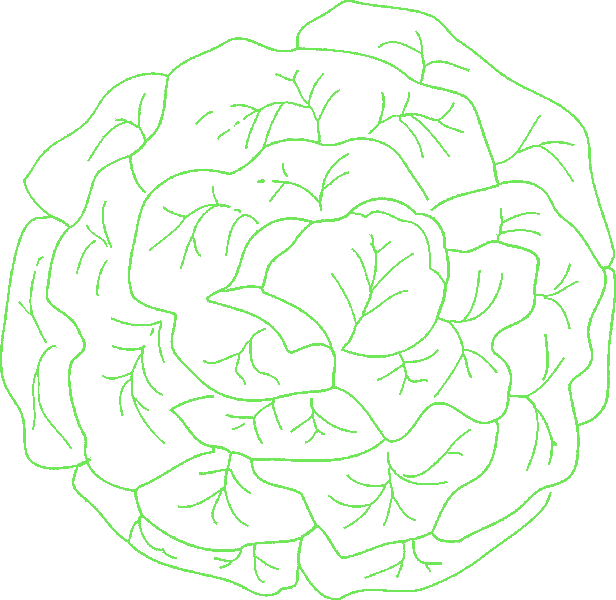
\includegraphics[height=.8\paperheight]{pics/saladeverte.png}};}
   %{\includegraphics[width=\paperwidth,height=\paperwidth]{/home/kodda/Dropbox/Bambi_notes/BambiDay_june2014/figs/haga.png}};}

\begin{frame}

\title{Computer vision for multiscale crop monitoring}

\author{david.colliaux@csl.sony.fr}
%\date{
       
%       \hspace{1cm}
%}
\titlepage

\vspace{.5cm}

\end{frame}

\usebackgroundtemplate{}

\begin{frame}{Multiscale view on crops}

\begin{columns}
\begin{column}{0.35\textwidth}

\begin{itemize}
\item Field
\item \alert{Crop bed}
\item \alert{Workspace}
\item {\color{romi} Plant}
\item \alert{Organ}
\item Cell
\item Molecular signals
\end{itemize}

\end{column}
\begin{column}{0.65\textwidth}
\hfill {\tiny \color{black!40}Photo by Noumena}
\cutpic{1cm}{5cm}{pics/FL02}\\
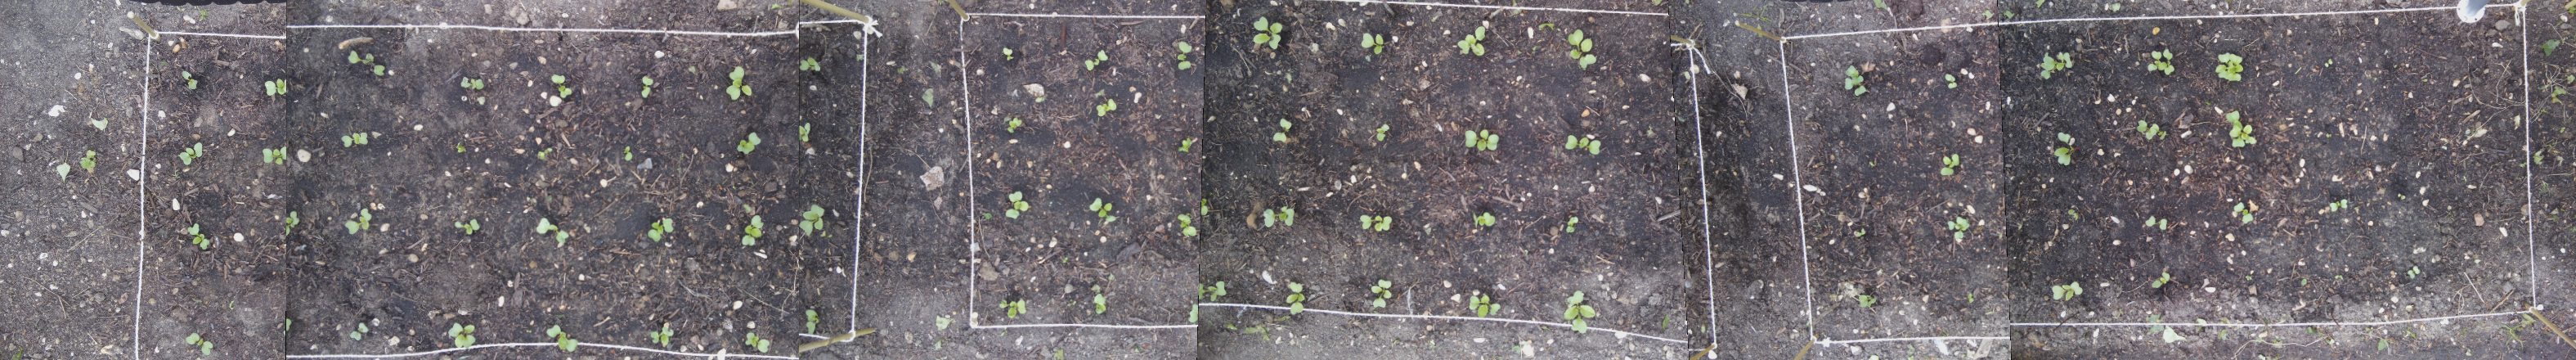
\includegraphics[width=\linewidth]{pics/cropbed.png}\\
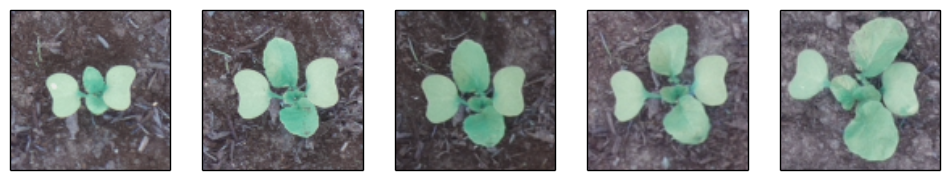
\includegraphics[width=\linewidth]{pics/growth.png}\\
\end{column}
\end{columns}

\end{frame}


\begin{frame}{Context: a robot...}%

\only<1>{
...for weeding...

\movie[label=mavideo,width=10cm,showcontrols,autostart]{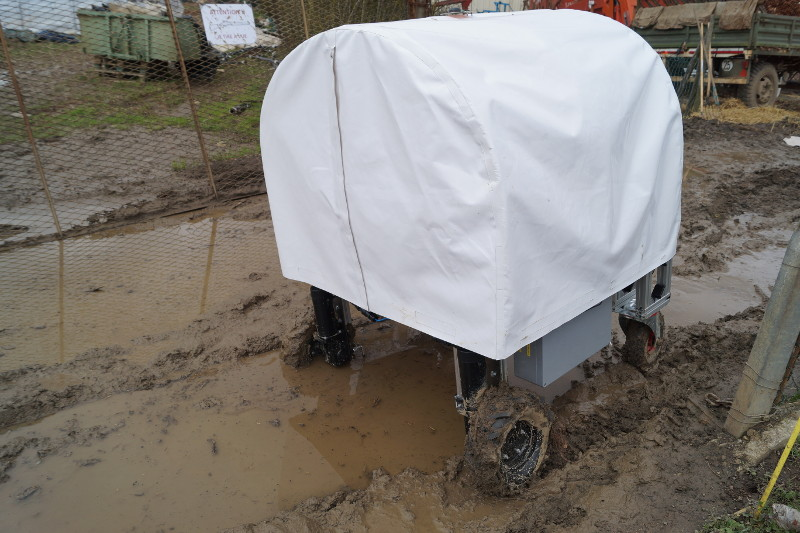
\includegraphics[width=.8\linewidth]{pics/lthink}}{weeding.mp4}\\%
}

\only<2-3>{
...for monitoring the growth of plants.

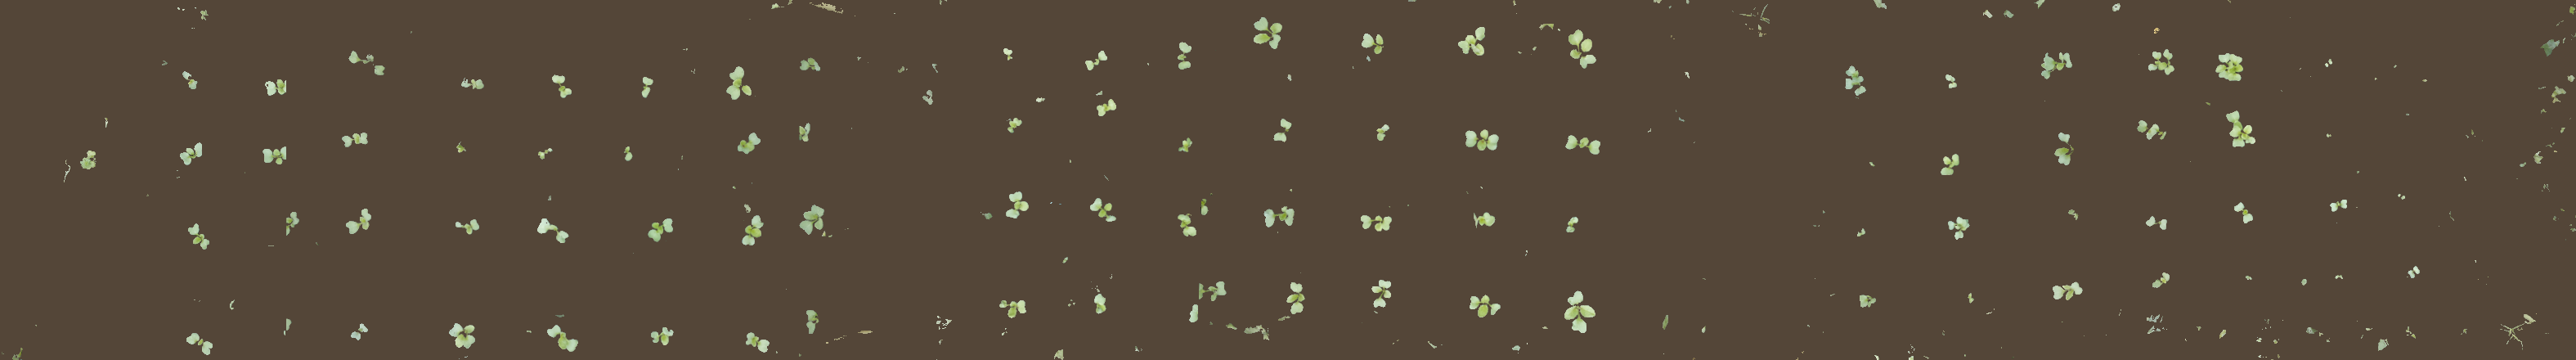
\includegraphics[width=\linewidth]{pics/cropbed_style2}\\

\movie[label=mavideo,width=4cm,showcontrols,autostart]{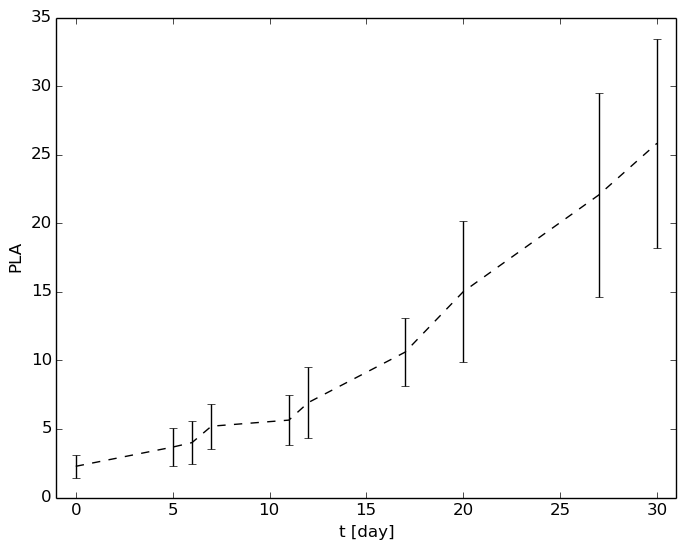
\includegraphics[width=.35\linewidth]{pics/PLAstat}}{pics/growth.mp4}
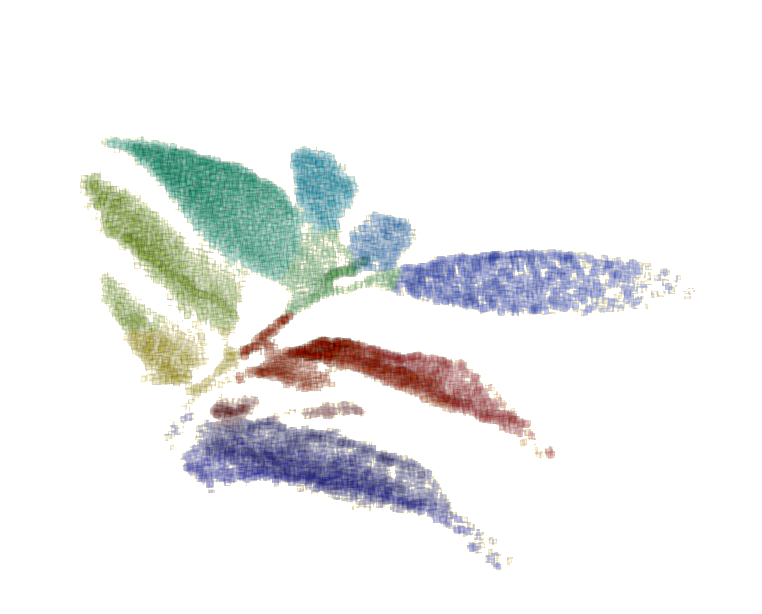
\includegraphics[width=.3\linewidth]{pics/seg_nobg}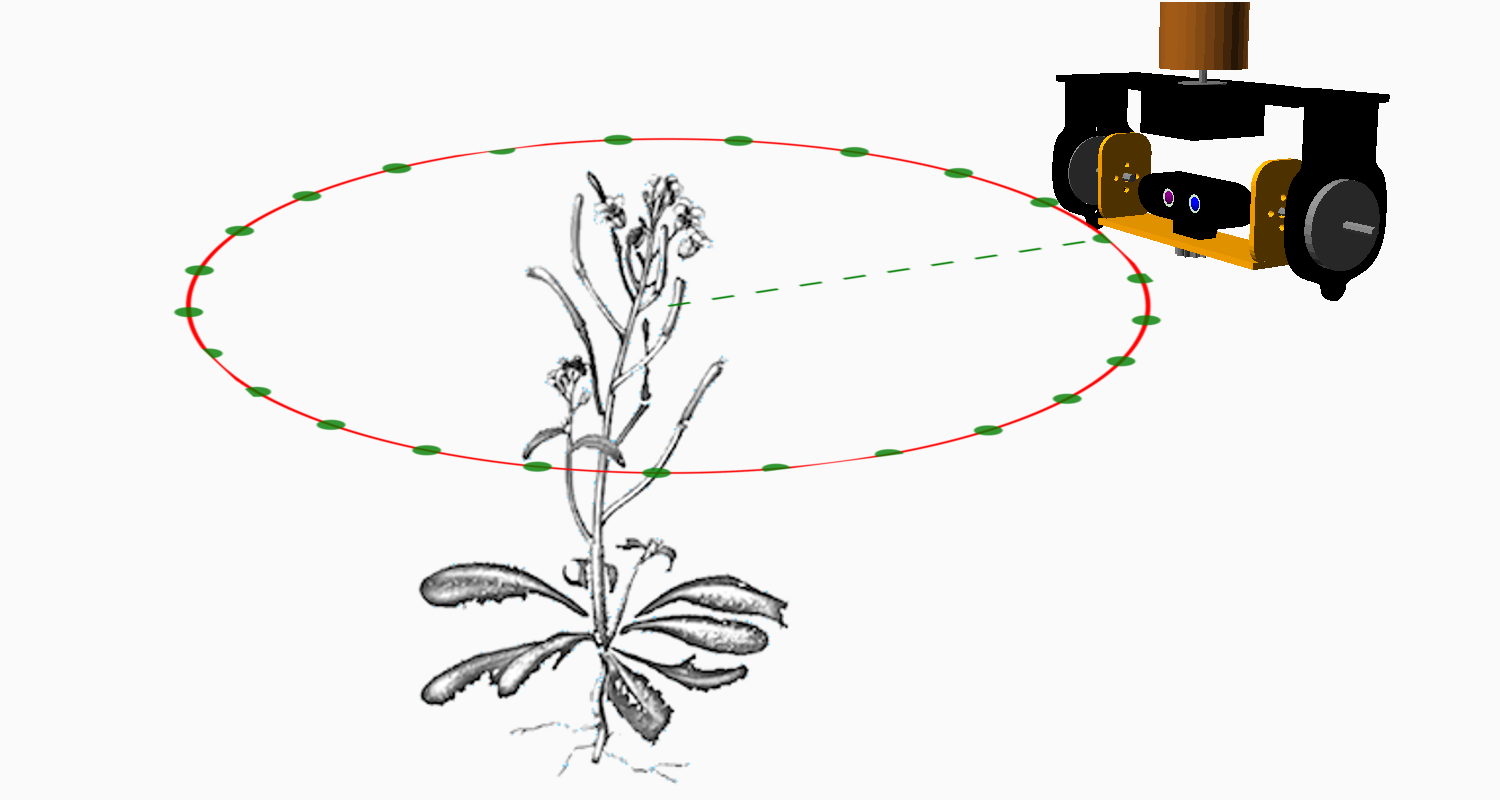
\includegraphics[width=.3\linewidth]{pics/scanner}\\
Growth dynamics
}

\only<2>{
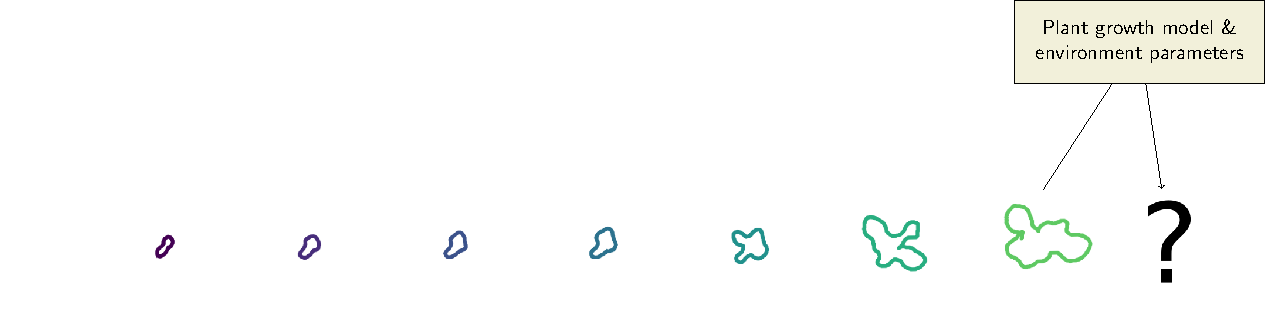
\includegraphics[width=\linewidth]{pics/trackSingle/guess.pdf}\\
}
\only<3>{
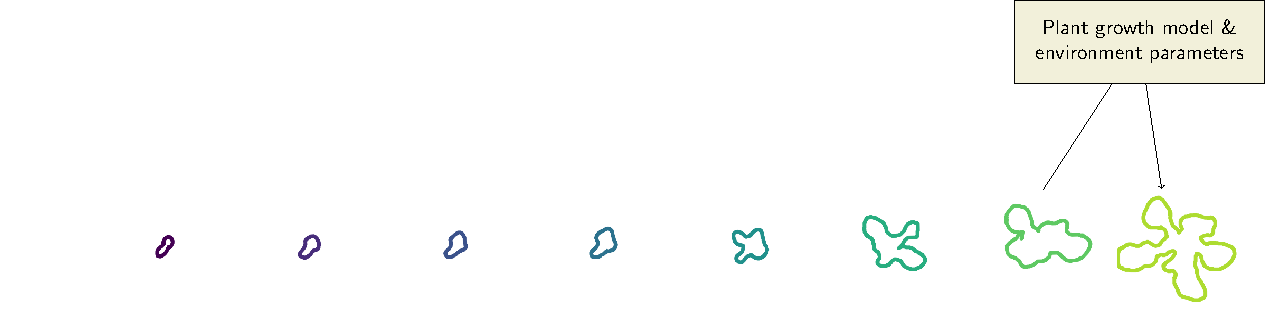
\includegraphics[width=\linewidth]{pics/trackSingle/pred0}\\
}

\end{frame}

\begin{frame}{Objectives of computer vision}%

\begin{columns}
\begin{column}{.5\linewidth}
\begin{itemize}
   \item<1-3> Segmentation
   \item<2-3> Mapping
   \item<3> Reconstruction (see also tomorrow)
\end{itemize}
\end{column}
\begin{column}{.5\linewidth}

\end{column}
\end{columns}

\end{frame}

 

\section{Segmentation}

\begin{frame}{Detecting plants on soil background.}

Defining a measure based on normalized RGB intensities:
\begin{columns}
\begin{column}{0.3\textwidth}

{\tiny
$$ExG=2{\color{green}G}-{\color{red}R}-{\color{blue}B}$$
$$CIVE = 0.441{\color{red}R} - 0.811{\color{green}G} + 0.385{\color{blue}B} + 18.787$$
$$MExG=1.262{\color{green}G}-0.884{\color{red}R}-0.311{\color{blue}B}$$}
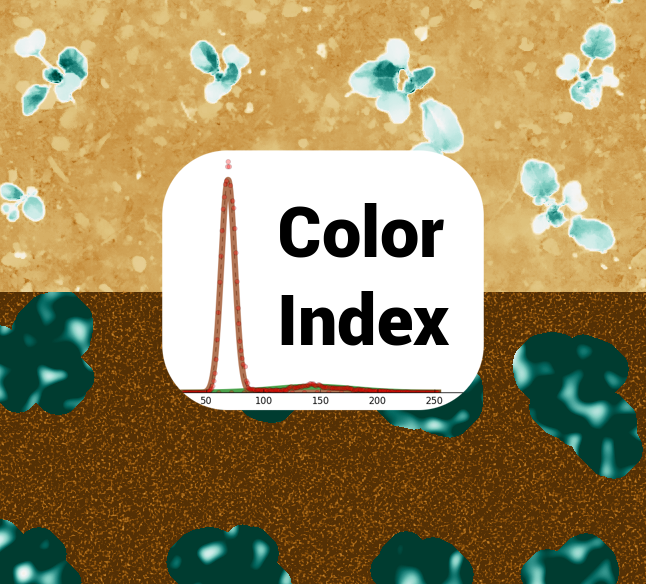
\includegraphics[width=\linewidth]{pics/seg}
\end{column}
\begin{column}{0.69\textwidth}
\begin{center}
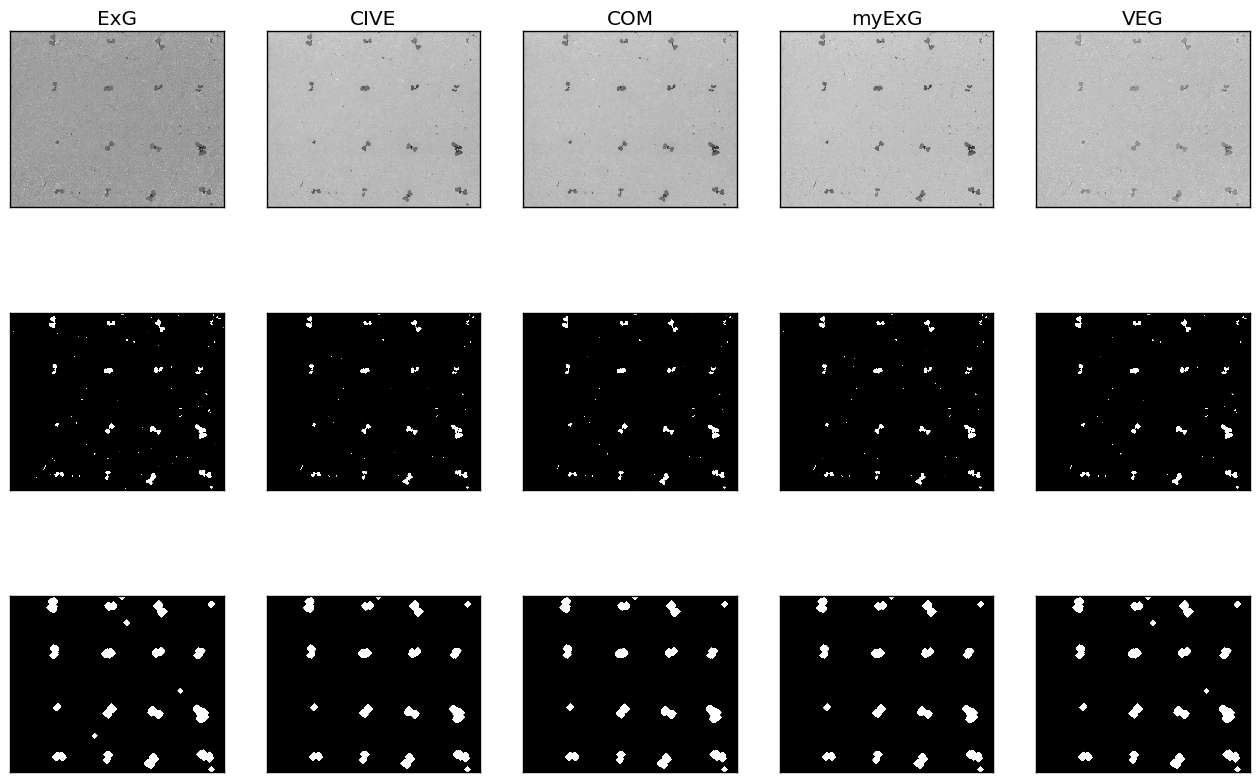
\includegraphics[width=\linewidth]{pics/cidx}
\end{center}
\end{column}
\end{columns}

Distributions with 2 well separated peaks: successful semgentation into background and plants (after filtering out the small patches)

{\tiny [Hamuda et al. A Survey of Image Processing Techniques for Plant Extraction and Segmentation in the Field. Comput. Electron. Agric., 2016]}

\end{frame}

\begin{frame}{Robustness of the segmentation segmentation.}

\begin{columns}
\begin{column}{0.45\textwidth}
\cutpic{2.5cm}{.8\linewidth}{pics/tpath}
\end{column}
\begin{column}{0.5\textwidth}
Usually sufficient to drive the weeding tool. 
\end{column}
\end{columns}

\begin{itemize}
\item Maybe limited for fine analysis of plant shapes.
\item Not robust to various light conditions or contexts.
\end{itemize}

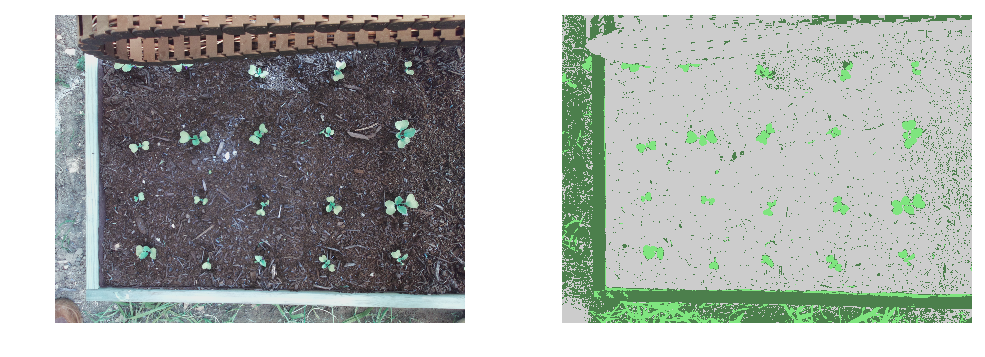
\includegraphics[width=.65\linewidth]{pics/mask_pb}
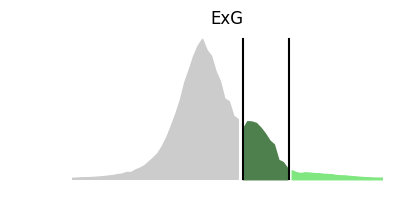
\includegraphics[width=.3\linewidth]{pics/trihist2}

=> use of annotated data

\end{frame}

\begin{frame}{Learning methods for segmentation.}

\begin{itemize}
\item Learned classifiers (Random forest, support vector machine) based on context, 
\item Convolutional neural network (SegNet). 
\end{itemize}

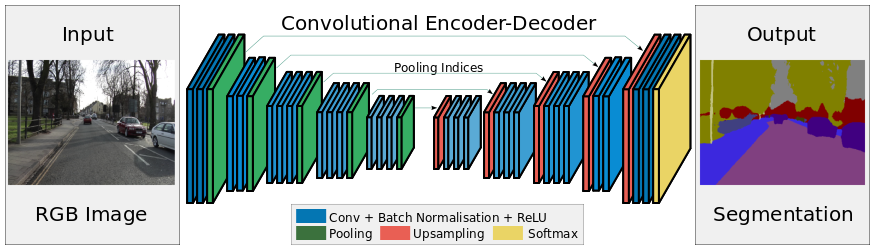
\includegraphics[width=\linewidth]{pics/segnet}

Dataset?

\hfill {\tiny  Vijay Badrinarayanan, Alex Kendall and Roberto Cipolla SegNet: A Deep Convolutional Encoder-Decoder Architecture for Image Segmentation. PAMI, 2017}
\end{frame}

\begin{frame}{Shortcuts for building datasets.}

\begin{columns}
\begin{column}{0.3\textwidth}
\begin{itemize}
\item External annotated datasets.
\item<2-3> Transfer knowledge fom generic networks
\end{itemize}
\end{column}
\begin{column}{0.65\textwidth}
\only<1>{
\begin{columns}
\begin{column}{0.3\textwidth}
{\tiny CVPPP 2017 Challenge}\\
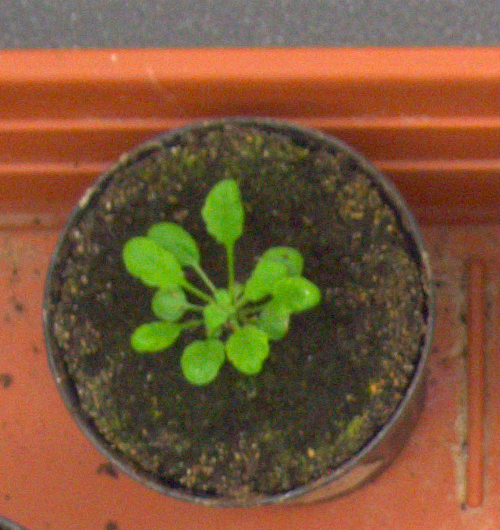
\includegraphics[width=\linewidth]{pics/rgb}\\

\includegraphics[width=\linewidth]{pics/fg}\\
\includegraphics[width=\linewidth]{pics/label} 
\end{column}
\begin{column}{0.65\textwidth}
{\tiny [Giselsson et al. A Public Image Database for Benchmark of Plant Seedling Classification Algorithms, 2017]}\\
\hfill 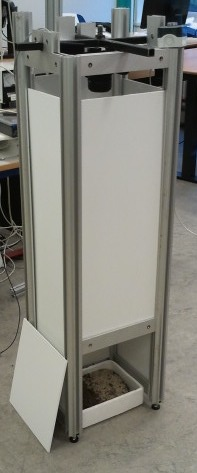
\includegraphics[width=.27\linewidth]{pics/rig}\\
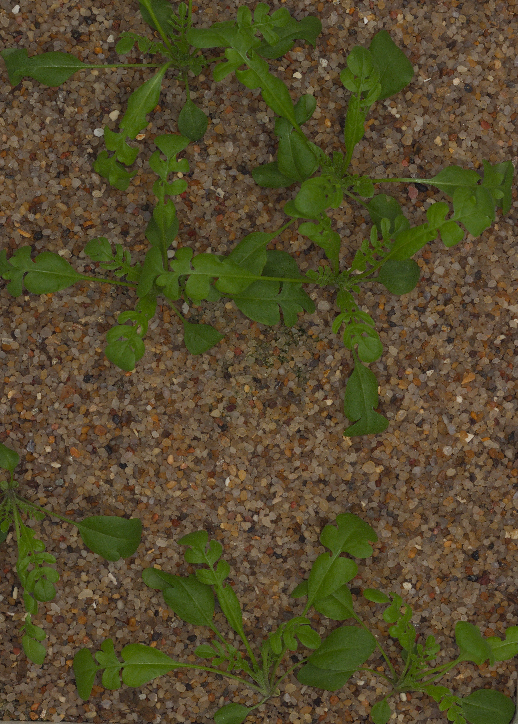
\includegraphics[width=.48\linewidth]{pics/pdata_rgb}
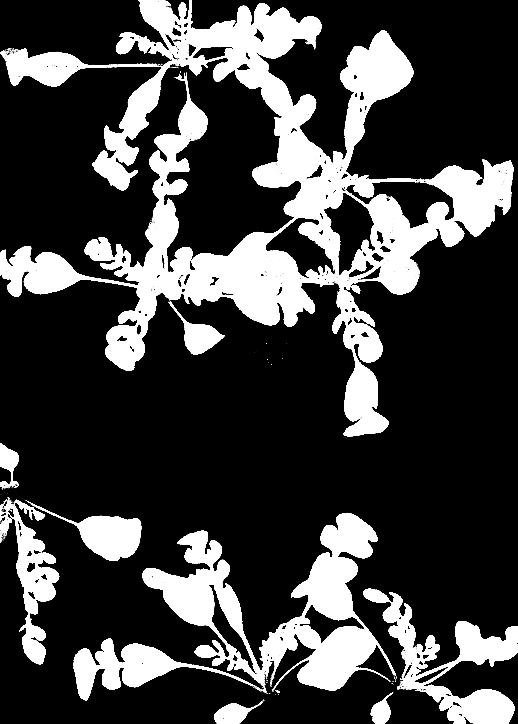
\includegraphics[width=.48\linewidth]{pics/pdata_fg}\\
\end{column}
\end{columns}

}
\only<2>{
Common objects in context (COCO) datset
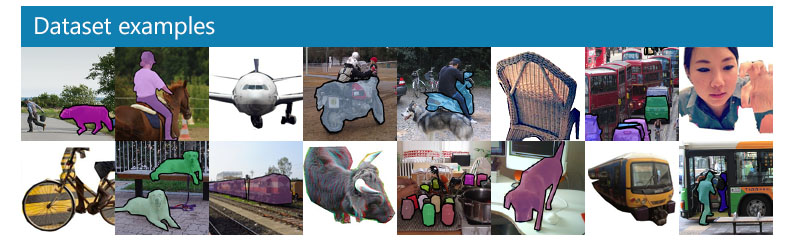
\includegraphics[width=\linewidth]{pics/coco-examples}
{\tiny Ren et al. Faster R-CNN: Towards Real-Time Object Detection with Region Proposal Networks, NIPS 2015}\\
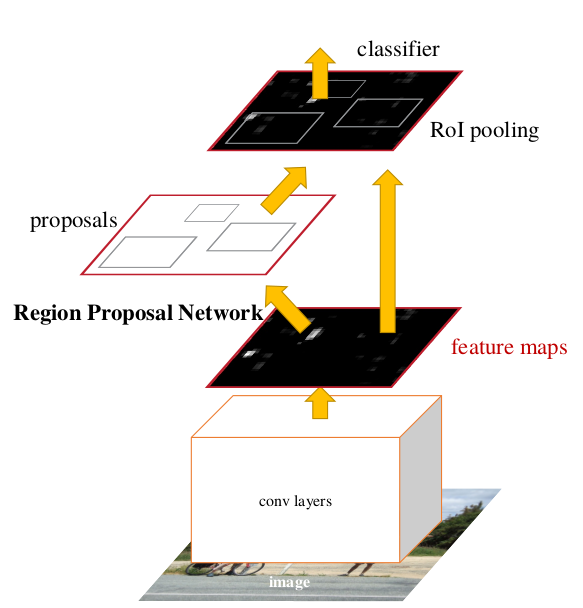
\includegraphics[width=.48\linewidth]{pics/fastrcnn}
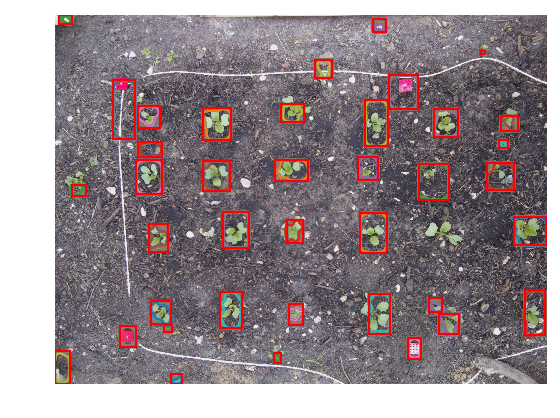
\includegraphics[width=.48\linewidth]{pics/frcnn_det}
}

\only<3>{
\begin{itemize}
\item Syntetic dataset
\item Building large datasets from few annotations (weakly supervised learning,...)
\includegraphics[width=\linewidth]{pics/data_curation}

\end{itemize}}
\end{column}
\end{columns}

\end{frame}


%\input{cropmonitoring} 

%\input{plantscan} 

\begin{frame}{Conclusion}

\begin{columns}
\begin{column}{0.5\textwidth}
Generic architecture

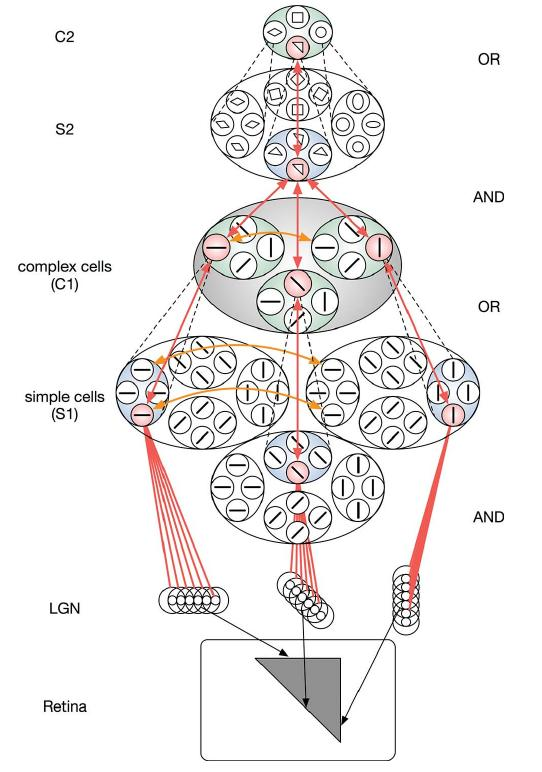
\includegraphics[width=\linewidth]{pics/hier}
\end{column}
\begin{column}{0.45\textwidth}

\begin{itemize}
\item Vision algorithms including models of the architecture and growth of plants.
\item Task specific algorithms (Deep learning: SegNet, PoseNet, MatchNet,...).
\end{itemize}

\end{column}
\end{columns}

\end{frame}


\end{document}
